% =====================================================================================
% Instance-BEq figures.  Regenerate ALL with:  bash scripts/figures/make_all_figures.sh
% Every figure is drawn ONLY from a real logged run (eval_logs/*.json); no mock numbers.
% Each block below records: source result file + the claim it supports (Experiment-Plan
% section / reviewer-rebuttal objection ID).  Reference each via \ref{} in the text.
% =====================================================================================

% --- FIG methods_f1 (CENTERPIECE) -------------------------------------------------------
% SOURCE: eval_logs/methods_vs_gold_result.json + ci_result.json (real unified scorer + bootstrap).
% CLAIM:  full 5-method x 4-check comparison; the certifier is exact on the two structural checks
%         and makes the fewest false certifications. Supports the head-to-head experiment.
\begin{figure*}[t]\centering
  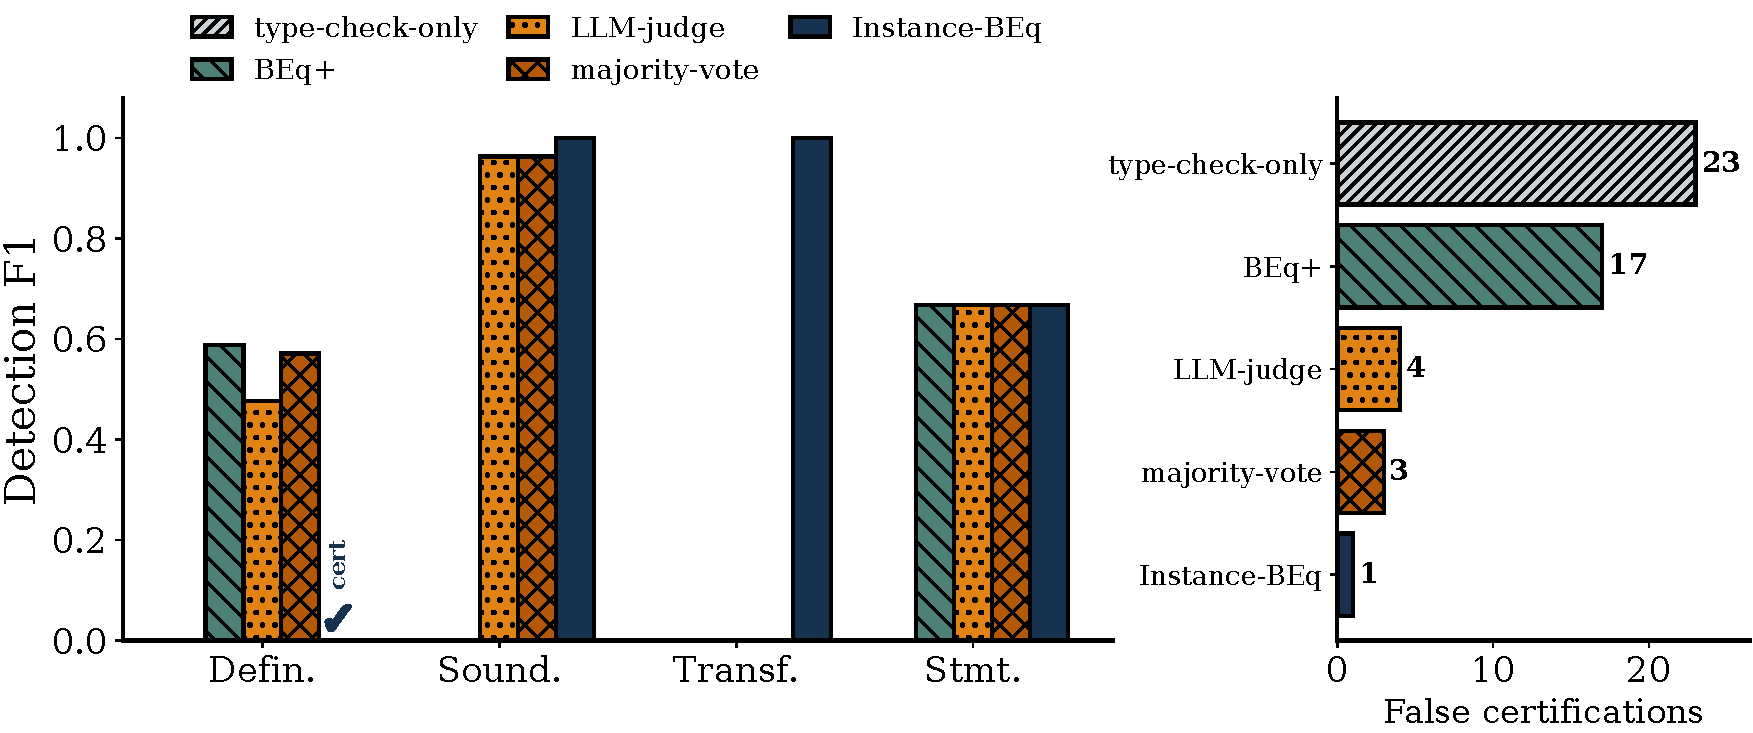
\includegraphics[width=\textwidth]{figures/methods_f1.pdf}
  \caption{(Left) per-check faithfulness-detection F1 for all five methods on the human gold;
  Instance-BEq is exact on instance soundness and is the only method with non-zero recall on
  transfer validity (on the definitional check it \emph{certifies} rather than detects, marked
  \textsc{cert}). (Right) false certifications---truly-unfaithful artifacts accepted as
  faithful---fall from 23 (type-check-only) to 1 (Instance-BEq, on the LLM statement bridge).}
  \label{fig:methodsf1}
\end{figure*}

% --- FIG ablations ----------------------------------------------------------------------
% SOURCE: eval_logs/ref_source_ablation_result.json + tactic_size_sweep_result.json (real).
% CLAIM:  check-1 coverage depends on reference source and ensemble size; precision is always 1.
\begin{figure}[t]\centering
  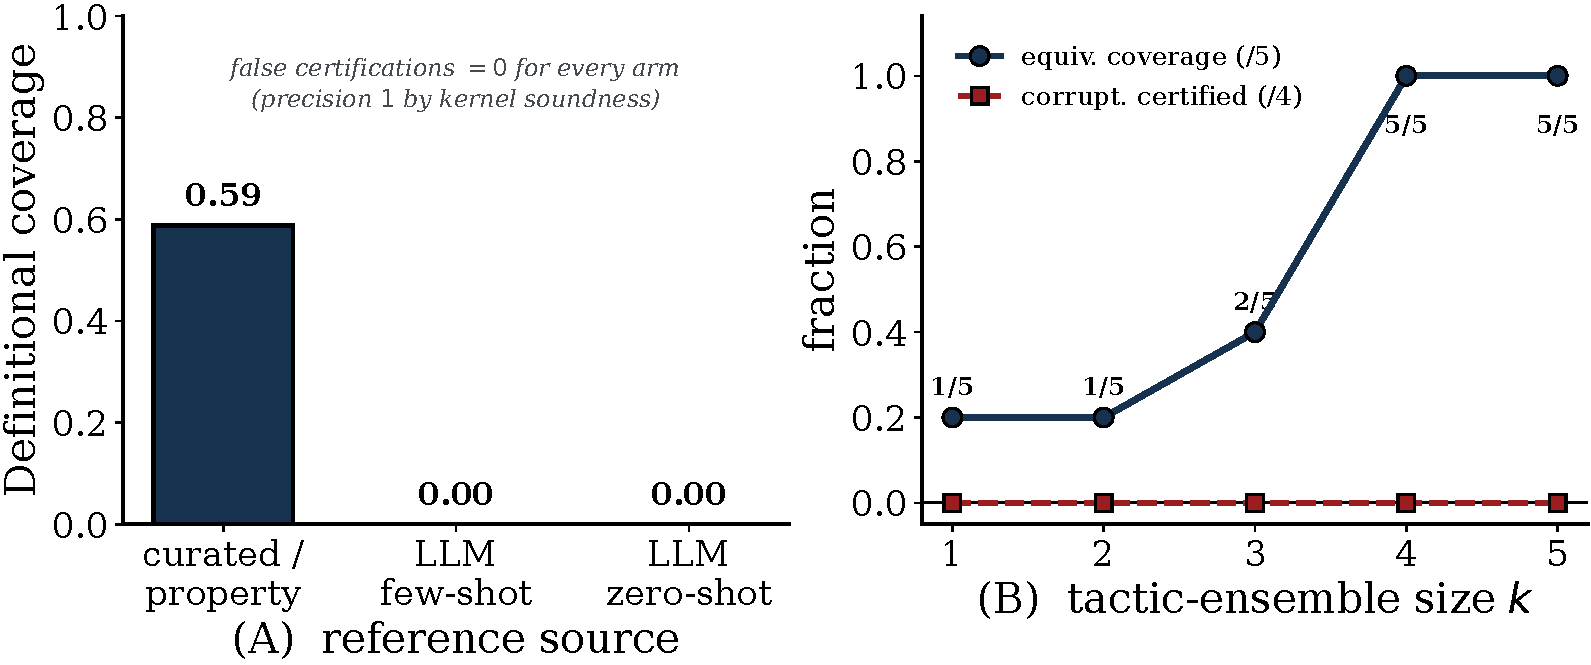
\includegraphics[width=\columnwidth]{figures/ablations.pdf}
  \caption{Check-1 ablations. (A) Definitional certification coverage by reference source: a
  curated/property reference recovers $59\%$ of faithful definitions, a 7B local model none;
  every arm makes zero false certifications. (B) Coverage on equivalent references grows with the
  tactic-ensemble size while false certifications on corruptions stay $0$ at every size.}
  \label{fig:ablations}
\end{figure}

% --- FIG prf_soundness ------------------------------------------------------------------
% SOURCE: eval_logs/soundness_methods_result.json  (assembled by scripts/soundness_all_methods.py
%         from fault_injection + certify_gold + llm_judge real runs).
% CLAIM:  EXPERIMENT_PLAN Section B (core P/R/F1 table) + REVIEWER_REBUTTAL R1 (type-check blind)
%         and R2 (LLM not formal): only the certifier is both exact and complete; baseline B
%         (majority-vote) is intentionally omitted (not yet run on real data).
\begin{figure}[t]\centering
  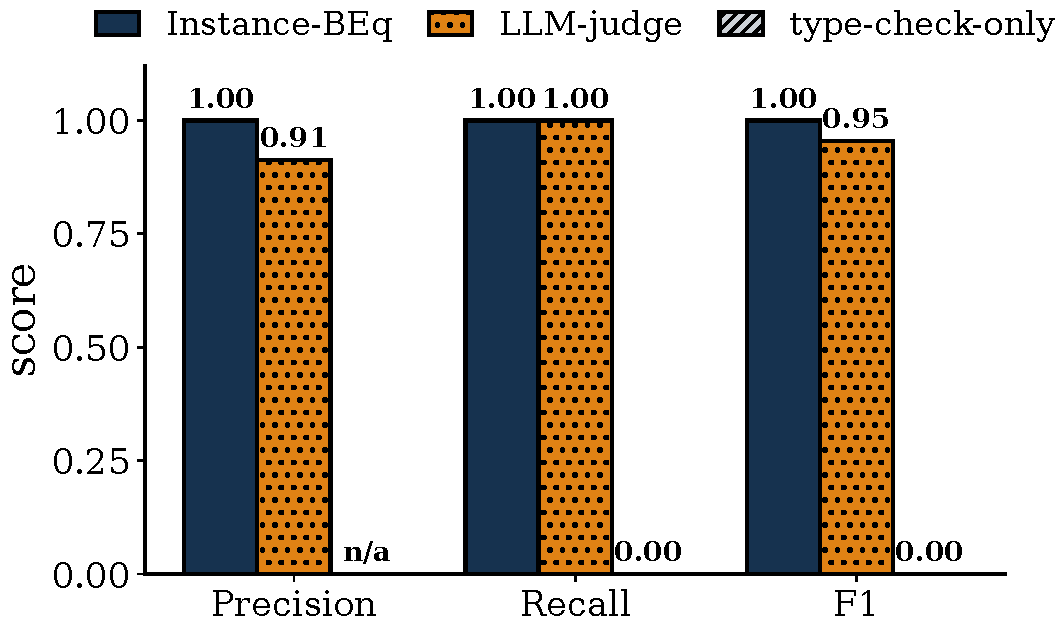
\includegraphics[width=\columnwidth]{figures/prf_soundness.pdf}
  \caption{Instance-BEq is the only method that detects hollow instances with both perfect
  precision and perfect recall, while type-check-only detects none.}
  \label{fig:prf}
\end{figure}

% --- FIG gold_hollow --------------------------------------------------------------------
% SOURCE: eval_logs/certify_gold_result.json + trace_fields_result.json + fault_injection_result.json
% CLAIM:  EXPERIMENT_PLAN Section C (motivating measurement) + REVIEWER_REBUTTAL R1: hollowness is
%         real, present in the authors' OWN gold examples, localized to named condition fields.
\begin{figure}[t]\centering
  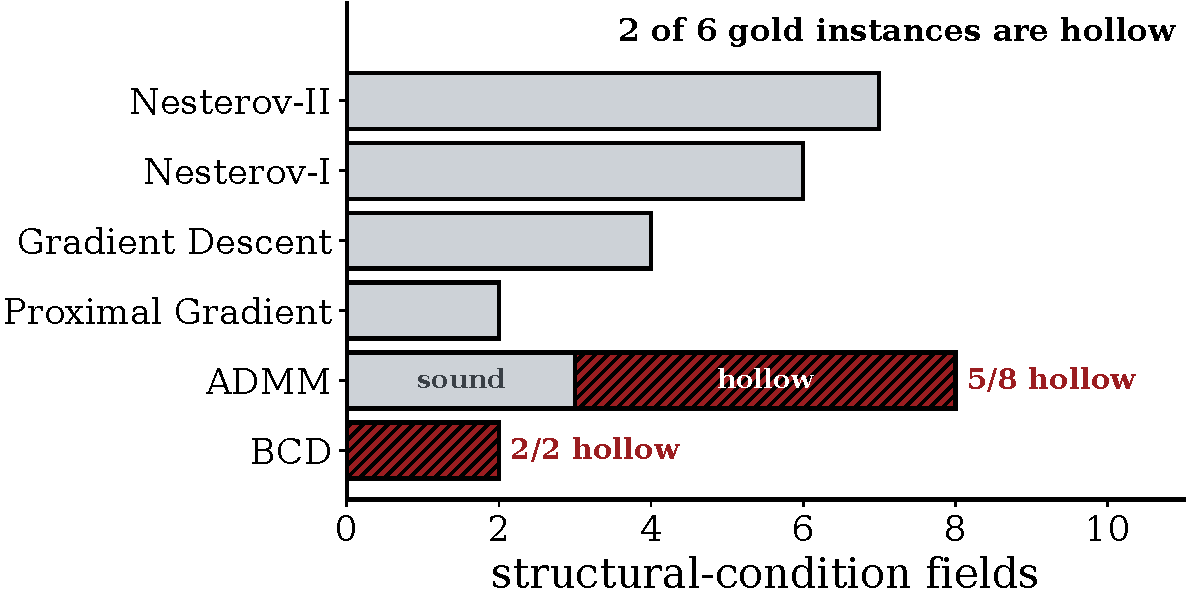
\includegraphics[width=\columnwidth]{figures/gold_hollow.pdf}
  \caption{Hollowness is not hypothetical: two of the six gold instances released with the base
  system leave structural-condition fields discharged by \texttt{sorry}.}
  \label{fig:goldhollow}
\end{figure}

% --- FIG check1_defeq -------------------------------------------------------------------
% SOURCE: eval_logs/check1_defeq_result.json
% CLAIM:  EXPERIMENT_PLAN Section B + Section D(1) (tactic ensemble, partial) + REVIEWER_REBUTTAL
%         R5/R7: check 1 proves equivalents and rejects corruptions; kernel-soundness => never a
%         false certification. (A full ensemble-SIZE ablation is not yet run.)
\begin{figure}[t]\centering
  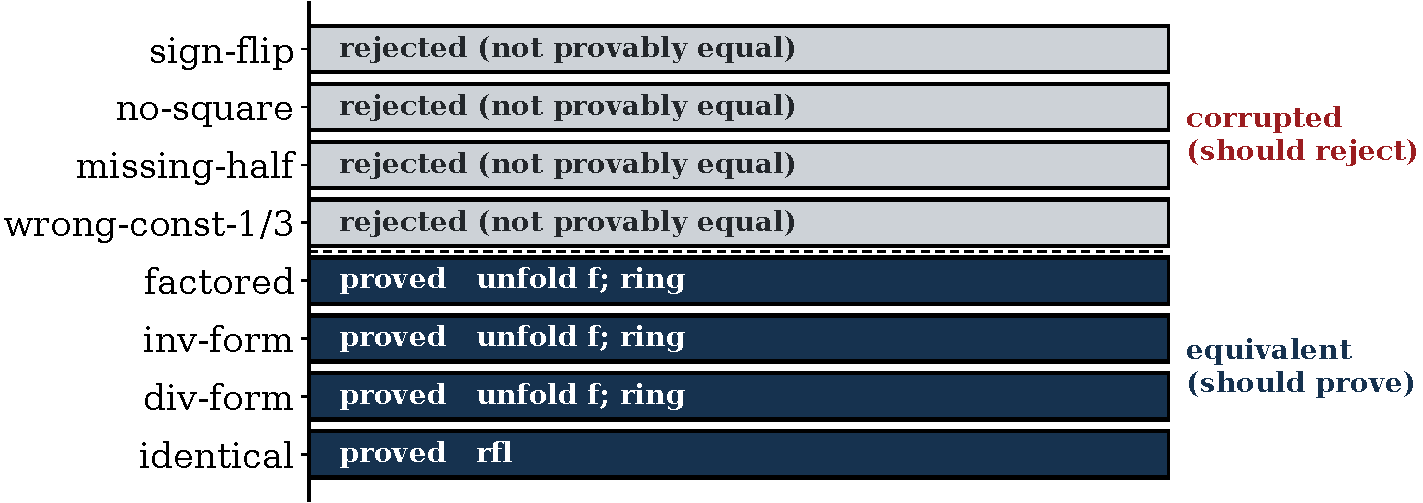
\includegraphics[width=\columnwidth]{figures/check1_defeq.pdf}
  \caption{Check~1 proves every semantically equivalent definition and rejects every corruption,
  so a certification is never false.}
  \label{fig:check1}
\end{figure}

% --- FIG catch_matrix (NOVEL) -----------------------------------------------------------
% SOURCE: eval_logs/soundness_methods_result.json
% CLAIM:  EXPERIMENT_PLAN Section B + REVIEWER_REBUTTAL R1 (type-check blind spot) & R2 (LLM
%         unreliability): per-instance correctness makes the failure modes visceral.
\begin{figure}[t]\centering
  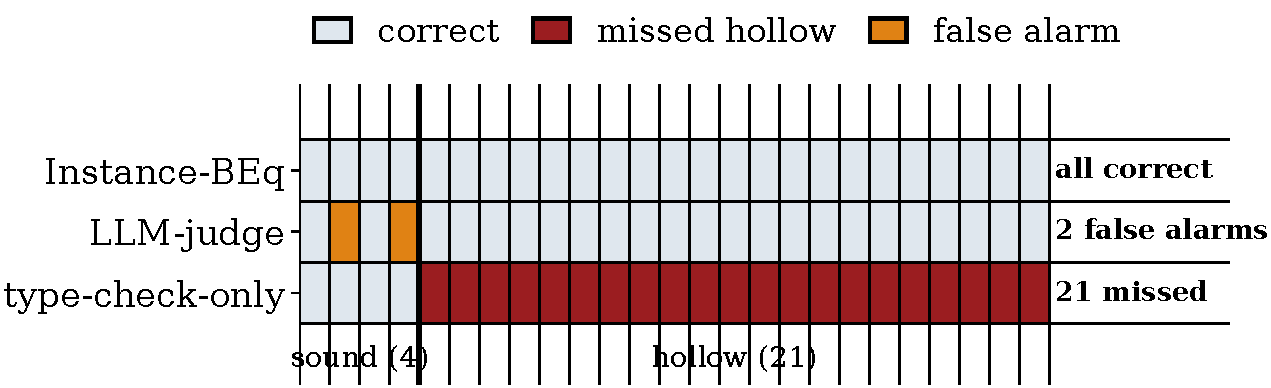
\includegraphics[width=\columnwidth]{figures/catch_matrix.pdf}
  \caption{Per instance, type-check-only misses every hollow case and the LLM-judge raises false
  alarms on sound ones, whereas Instance-BEq is correct on all 25.}
  \label{fig:catch}
\end{figure}

% --- FIG pr_tradeoff (NOVEL) ------------------------------------------------------------
% SOURCE: eval_logs/soundness_methods_result.json  (F1 iso-contours are analytic, not data)
% CLAIM:  EXPERIMENT_PLAN Section B + REVIEWER_REBUTTAL R2/R5: the symbolic certifier dominates the
%         precision-recall plane; baselines each forfeit one axis.
\begin{figure}[t]\centering
  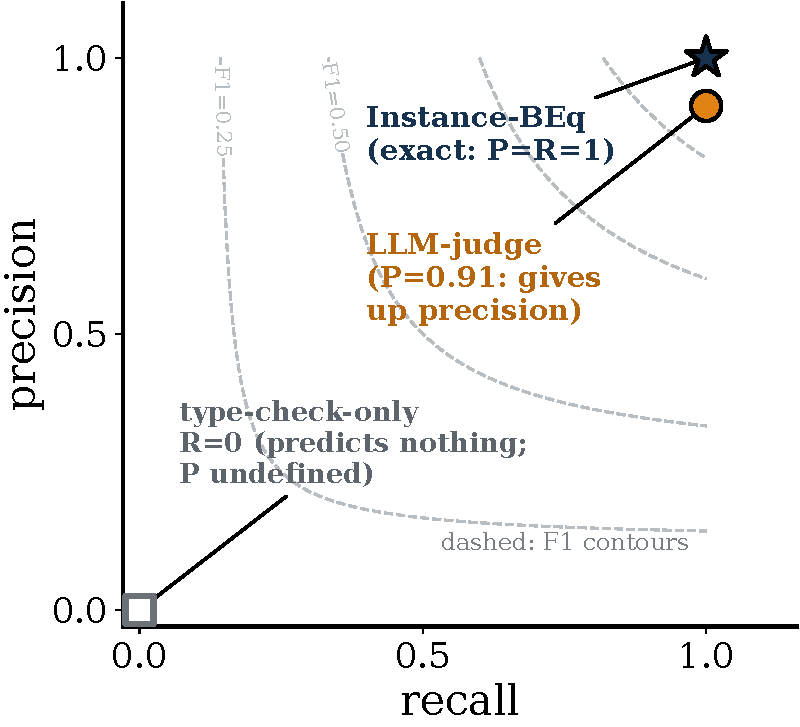
\includegraphics[width=0.86\columnwidth]{figures/pr_tradeoff.pdf}
  \caption{Instance-BEq sits alone at the $(1,1)$ corner; the LLM-judge concedes precision and
  type-check-only concedes all recall.}
  \label{fig:prtradeoff}
\end{figure}

% --- FIG tau_human ----------------------------------------------------------------------
% SOURCE: eval_logs/methods_vs_gold_result.json (gold.jsonl + llm_judge_gold_result.json +
%         soundness_gate_result.json + human_vs_expert.json — all real).
% CLAIM:  EXPERIMENT_PLAN Section B (human-correlation) + REVIEWER_REBUTTAL R2: the LLM-judge's
%         agreement with human labels falls below the inter-annotator ceiling on the hard
%         (definitional, transfer) checks; the formal certifier is exact where decidable.
\begin{figure}[t]\centering
  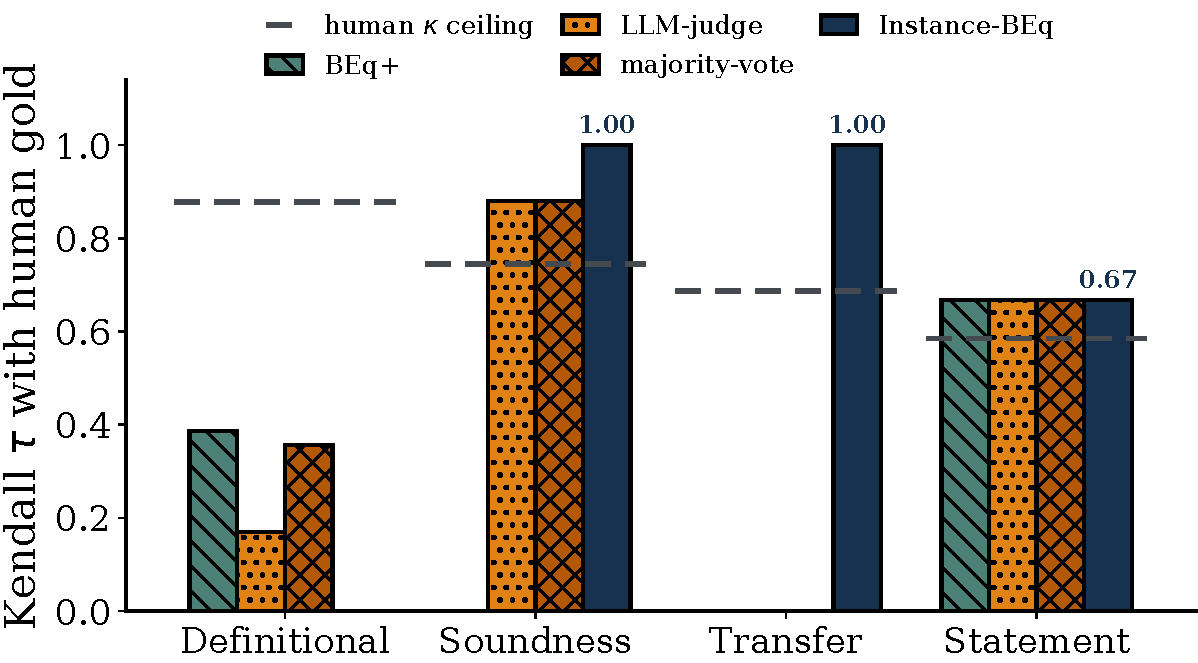
\includegraphics[width=\columnwidth]{figures/tau_human.pdf}
  \caption{The LLM-judge correlates with human judgement well below the inter-annotator ceiling on
  the definitional and transfer checks, whereas Instance-BEq is exact ($\tau{=}1$) where the check is
  decidable and type-check-only is blind everywhere.}
  \label{fig:tauhuman}
\end{figure}

% --- FIG calibration --------------------------------------------------------------------
% SOURCE: eval_logs/llm_judge_gold_result.json (real; per-item confidence + correctness).
% CLAIM:  EXPERIMENT_PLAN Section D(6) (calibration of the LLM-assisted path) + R2: the LLM-judge is
%         miscalibrated (ECE 0.179) — its most-used "certain" rating is still wrong 14% of the time.
\begin{figure}[t]\centering
  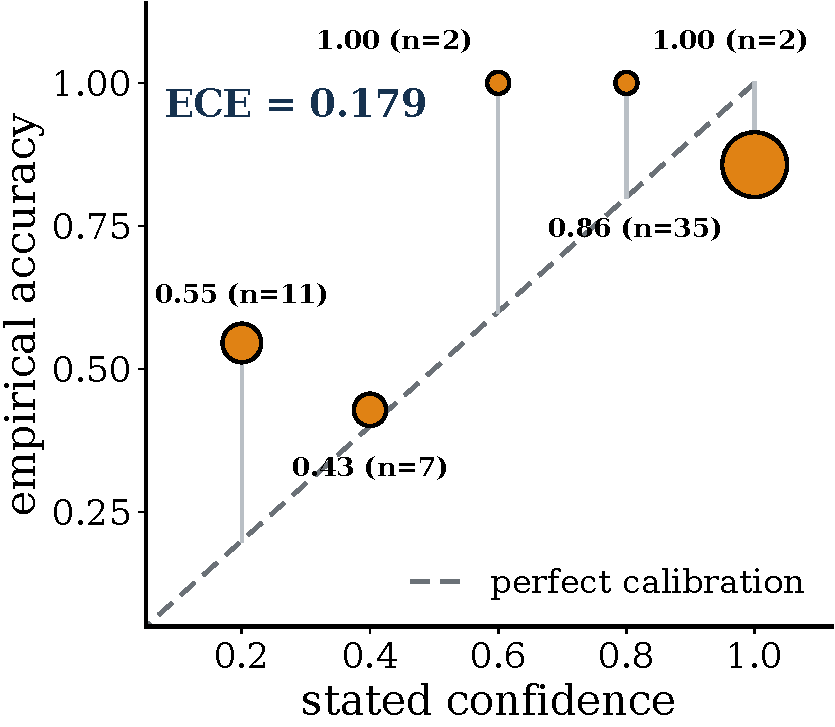
\includegraphics[width=0.86\columnwidth]{figures/calibration.pdf}
  \caption{The LLM-judge is miscalibrated (ECE $=0.179$): its confidence does not track its accuracy,
  and its most-used maximal-confidence rating is still wrong 14\% of the time.}
  \label{fig:calibration}
\end{figure}

% =====================================================================================
% All planned figures are now produced from real logged runs:
%   * Reference-def-source ablation (curated/property vs few-shot vs zero-shot 7B) -> Fig. ablations(A).
%   * Tactic-ensemble-SIZE ablation (1->full coverage@k sweep)                     -> Fig. ablations(B).
%   * Five-method x four-check head-to-head + false-certification safety panel      -> Fig. methodsf1.
% =====================================================================================
